%%%%%%%%%%%%%%%%%%%%% chapter.tex %%%%%%%%%%%%%%%%%%%%%%%%%%%%%%%%%
%
% sample chapter
%
% Use this file as a template for your own input.
%
%%%%%%%%%%%%%%%%%%%%%%%% Springer-Verlag %%%%%%%%%%%%%%%%%%%%%%%%%%

\chapstarthook{The content of this chapter corresponds with the
following publication: \textbf{J.A. Aguilar, I. Garrig{\'o}s, J.-N. Maz{\'o}n, J. Trujillo. An MDA Approach for Goal-oriented Requirement Analysis in Web Engineering. Journal of Universal Computer Science (J.UCS), 16(17): 2475-2494 (2010).}}


\chapter{An MDA Approach for Goal-oriented Requirement Analysis in Web Engineering}
\label{c4} % Always give a unique label
% use \chaptermark{}
% to alter or adjust the chapter heading in the running head

Since the previous chapter has defined how to obtain a
relational-based implementation of the multidimensional conceptual
model, this chapter focuses on obtaining a logical representation
directly based on multidimensional technology, thus showing the full
potential of applying formal transformations within a model-driven
approach. The content of this chapter corresponds with the part of
the approach shaded in the figure below.

%\begin{figure}[h!]
%  \begin{center}
%    \includegraphics[width=0.7\textwidth]{img/chapters/chapter4}
%  \end{center}
%  %\caption{} \label{}
%\end{figure}


This chapter was published in the \emph{International Conference on
Data Warehousing and Knowledge Discovery (DaWaK)}. This conference
has become one of the most important international scientific events
through which to bring together researchers, developers and
practitioners to discuss the latest research issues and experiences
in developing and deploying data warehousing and knowledge discovery
systems, applications, and solutions. Each year, \emph{DaWaK} seeks
to introduce innovative principles, methods, algorithms and
solutions to challenging problems faced in the development of data
warehousing, knowledge discovery and data mining applications.
\emph{DaWaK} is, therefore, a leading international forum for the
presentation and discussion of current research and applications in
which the major emphasis is on data warehousing. The high quality of
this conference can be demonstrated through the following two facts:
the \emph{acceptance rate} of this conference is usually around
\emph{30\%}, and the \emph{Estimated Impact of Conference (EIC)} is
\emph{0.86} according to \emph{The Computer Science Conference
Ranking Website}
(\url{http://www.cs-conference-ranking.org/home.html}).


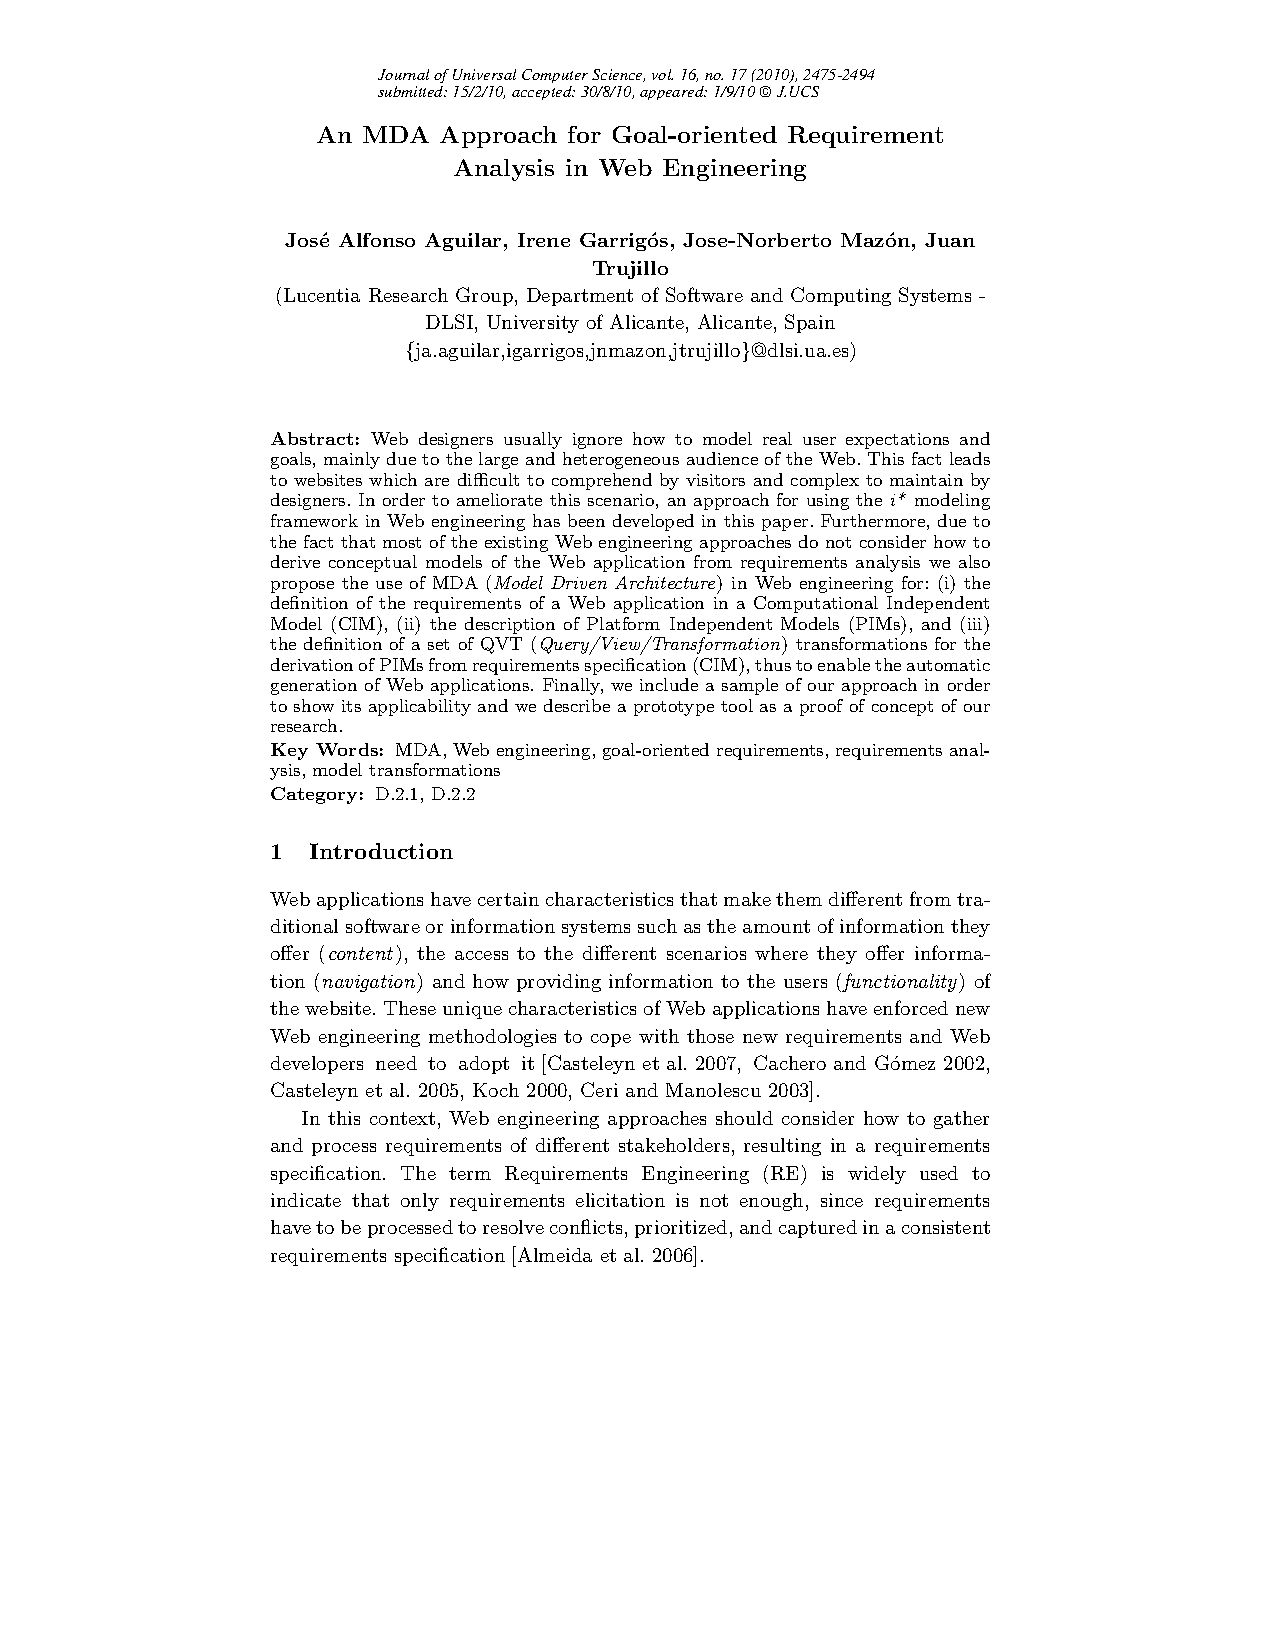
\includepdf[openright=true,pages={1-20}]{papers/JUCS2010.pdf}
%
